\documentclass[tikz]{standalone}
\usepackage[outline]{contour}

\begin{document}
	    \contourlength{1.5pt}
	    	    \tikzset{
	    	double arrow/.style args={#1 colored by #2 and #3}{
	    		-stealth,line width=#1,#2, % first arrow
	    		postaction={draw,-stealth,#3,line width=(#1)/3,
	    			shorten <=(#1)/3,shorten >=2*(#1)/3}, % second arrow
	    	}
	    }
\begin{tikzpicture}
    \node[anchor=south west,inner sep=0] at (0,0) {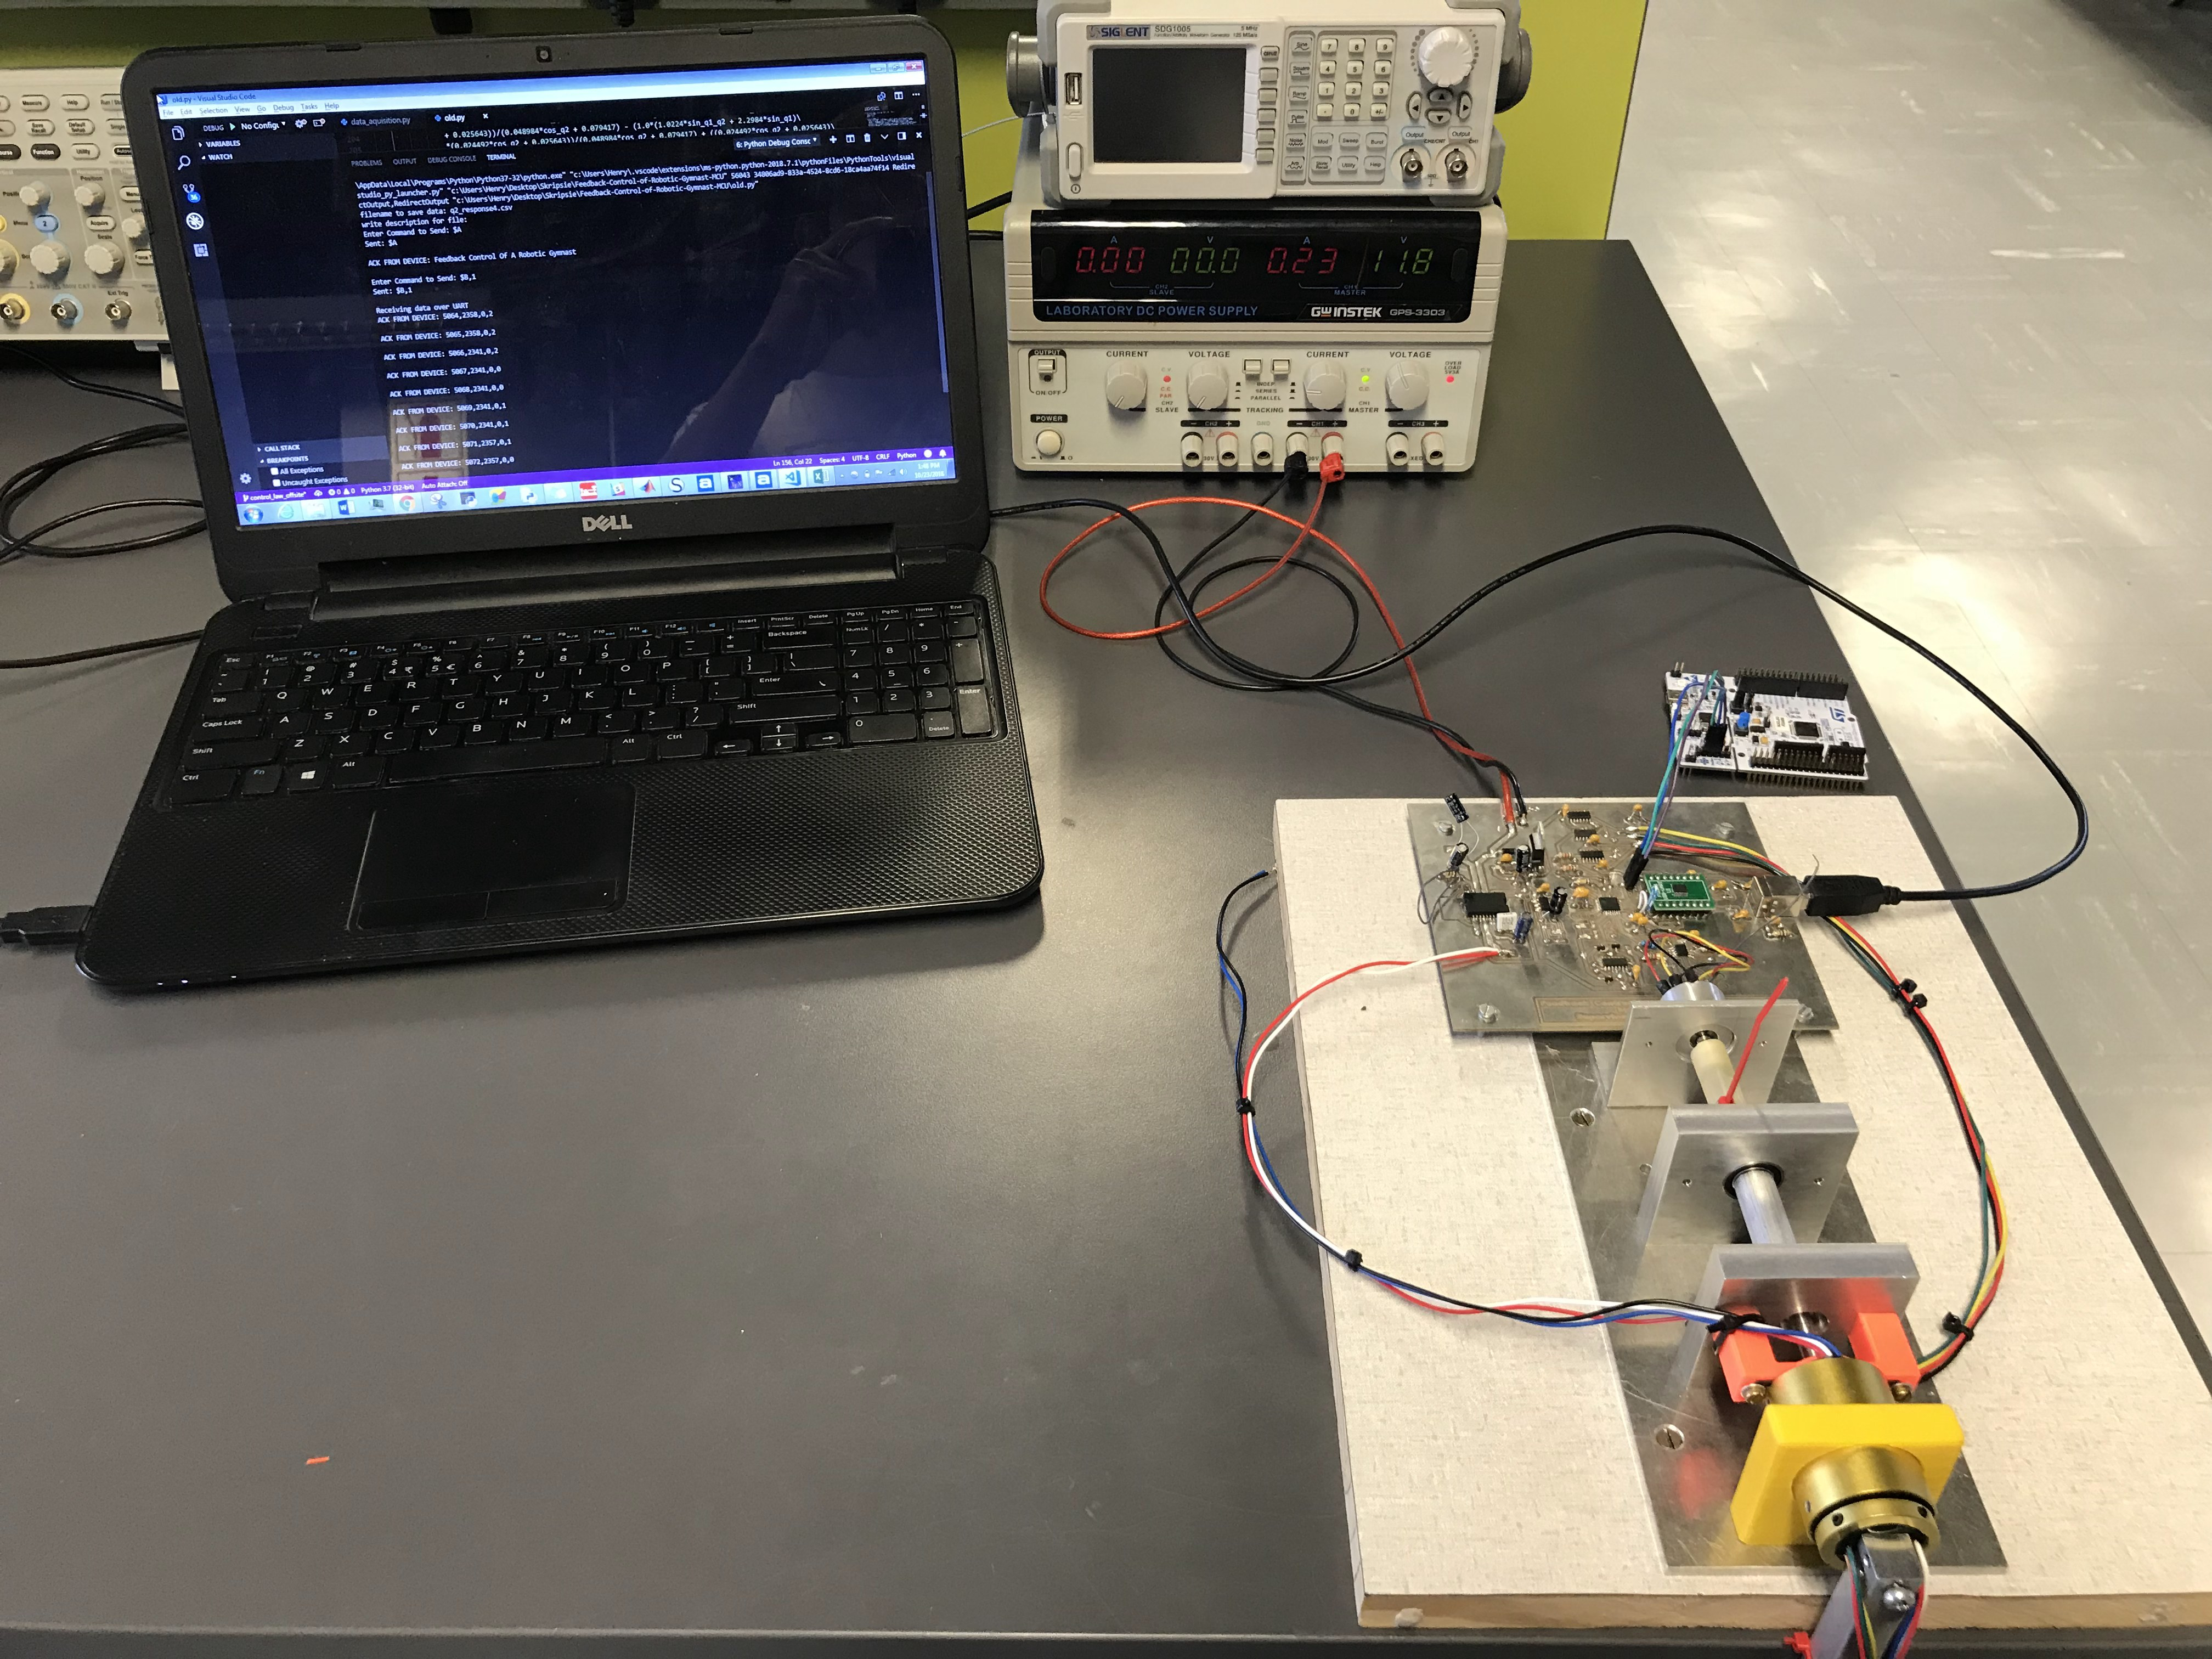
\includegraphics[width=\textwidth]{elec_sys.jpg}};
    %microcontroller
    %\draw[green,ultra thick,rounded corners] (6.5,5) node[above]{ \textbf{MCU} };
    

    
    \node[black] at (9,5.8) {\contour{white}{\textbf{PCB}}};
    \draw[yellow,ultra thick,rounded corners] (7.5,3.5) rectangle (10.5,5.5);
    
    %Mechanical

    
    %PC
    \node[black] at (3,3.5) {\contour{white}{\textbf{External Computer}}};
    \draw[yellow,ultra thick,rounded corners] (0.7,3.2) rectangle (5.3,9);
    
    % Power
    \draw[yellow,ultra thick,rounded corners] (5.5,6.5) rectangle (8.5,8);
    \node[black] at (7,8.2) {\contour{white}{\textbf{Bench Power Supply}}};

    
    %Mechan
    \draw[yellow,ultra thick,rounded corners] (9,0.5) rectangle (10.5,3.2);
    \node[rotate=0,black] at (9.5,1) {\contour{white}{\textbf{Mechanical Hardware}}};
    

    
\end{tikzpicture}
\end{document}